\begin{name}
{Đề Ôn Tập HS TB-Yếu}
{Năm học 2025-2026}
\end{name}

\Opensolutionfile{ans}[ans/De-TB-Yeu-So-16]
\cautn
\begin{ex}
	Cho hàm số $y=2^x$ có đồ thị là đường cong trong hình bên. Diện tích $S$ của hình phẳng trong hình bằng
	\begin{center}
		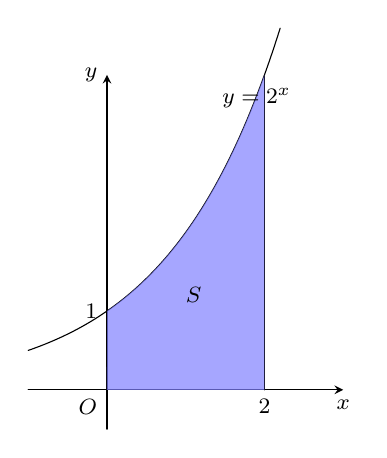
\begin{tikzpicture}[scale=1, font=\footnotesize, line join=round, line cap=round, >=stealth,declare function={f(\x)=2^(\x);}]
			\draw[->] (-1,0)--(3,0) node[below] {$x$};
			\draw[->] (0,-0.5)--(0,4) node[left] {$y$};
			\draw[domain=-1:2.2,samples=100,smooth] plot (\x,{f(\x)});
			\draw (0,0) node[below left] {$O$};
			\draw (2,0)--(2,{f(2)});
			\draw (0,0)--(2,0);
			\fill[blue!50,opacity=0.7] (0,0)--(2,0)--(2,{f(2)})--plot[domain=2:0,samples=100] (\x,{f(\x)})--cycle;
			\node at (1.1,1.2) {$S$};
			\node at (1.9,3.7) {$y=2^x$};
			\node at (2,0) [below] {$2$};
			\node at (0,1) [left] {$1$};
		\end{tikzpicture}
	\end{center}
	\choice
	{$S=\displaystyle\int \limits_{1}^{2}2^x\mathrm{\,d}x$}
	{\True $S=\displaystyle\int \limits_{0}^{2}2^x\mathrm{\,d}x$}
	{$S=\displaystyle\int \limits_{0}^{2}2^{2x}\mathrm{\,d}x$}
	{$S=\pi\displaystyle\int \limits_{0}^{2}2^x\mathrm{\,d}x$}
	\loigiai{
		Diện tích $S$ của hình phẳng trong hình trên bằng $S=\displaystyle\int \limits_{0}^{2}2^x\mathrm{\,d}x$.
	}
\end{ex}

\begin{ex}
	Cho hai biến cố $A$ và $B$ có $\mathrm{P}(A)=0{,}3$, $\mathrm{P}(B)=0{,}6$, $\mathrm{P}(A\cap B)=0{,}2$. Xác suất $\mathrm{P}(A\mid B)$ là
	\choice
	{$\dfrac{1}{2}$}
	{$\dfrac{1}{6}$}
	{$\dfrac{2}{3}$}
	{\True $\dfrac{1}{3}$}
	\loigiai{
		Theo định nghĩa xác suất có điều kiện ta có $\mathrm{P}(A\mid B)=\dfrac{\mathrm{P}(A\cap B)}{\mathrm{P}(B)}=\dfrac{0{,}2}{0{,}6}=\dfrac{1}{3}$.
	}
\end{ex}

\begin{ex}
	Cho hàm số $y=f(x)$ có đồ thị như hình vẽ sau
	\begin{center}
		\begin{tikzpicture}[declare function={a=1; b=2; c=3;}]
			\path
			(0,0) coordinate (O)
			(c,0) coordinate (X)
			(0,c) coordinate (Y)
			(-a,0) coordinate (A)
			(a,0) coordinate (B)
			(-a,-b) coordinate (C)
			(a,-b) coordinate (D);
			
			\draw[->] (-c,0)--(c,0);
			\draw[->] (0,-c)--(0,c);
			
			\draw[dashed] (A)--(C)--(D)--(B);
			
			\clip (-2,-3) rectangle (1.6,2.5);
			\draw[domain=-1.6:1.6,smooth] plot (\x,{4*(\x)^4-8*(\x)^2+2});
			
			\node[font=\footnotesize] at (-1,0.25) {$-1$};
			\node[font=\footnotesize] at (1,0.25) {$1$};
			\node[font=\footnotesize] at (-0.3,2) {$2$};
			\node[font=\footnotesize] at (-0.35,-2.2) {$-2$};
			
			\node[font=\footnotesize] at (c,0.25) {$x$};
			\node[font=\footnotesize] at (0,c) {$y$};
		\end{tikzpicture}
	\end{center}
	Giá trị cực đại của hàm số bằng
	\choice
	{$0$}
	{\True $2$}
	{$-1$}
	{$1$}
	\loigiai{ }
\end{ex}

\begin{ex}
	Tập nghiệm bất phương trình $2^x>8$ là
	\choice
	{$\left(-\infty;3\right)$}
	{$\left(-\infty;3\right]$}
	{$\left[3;+\infty\right)$}
	{\True $\left(3;+\infty\right)$}
	\loigiai{
		Ta có $2^x>8\Leftrightarrow 2^x>2^3\Leftrightarrow x>3$.\\
		Vậy tập nghiệm của bất phương trình là $\left(3;+\infty\right)$.
	}
\end{ex}

\begin{ex}
	Tất cả các nguyên hàm của hàm số $f(x)=3^{-x}$ là
	\choice
	{$-3^{-x}+C$}
	{$\dfrac{3^{-x}}{\ln 3}+C$}
	{$3^{-x}\ln 3+C$}
	{\True $-\dfrac{3^{-x}}{\ln 3}+C$}
	\loigiai{
		Ta có $\displaystyle\int 3^{-x}\mathrm{\,d}x=-\dfrac{3^{-x}}{\ln 3}+C$.
	}
\end{ex}

\begin{ex}
	Khối lăng trụ có thể tích là $3a^3$ và chiều cao bằng $3a$. Khi đó diện tích đáy của khối lăng trụ là
	\choice
	{\True $a^2$}
	{$\dfrac{1}{3}a^2$}
	{$3a^2$}
	{$a$}
	\loigiai{
		Ta có $V=B\cdot h\Rightarrow B=\dfrac{V}{h}=\dfrac{3a^3}{3a}=a^2$.
	}
\end{ex}

\begin{ex}
	Cho hàm số $y=f(x)$ có bảng biến thiên như hình vẽ sau
	\begin{center}
		
\begin{tikzpicture}
			\tkzTabInit[nocadre=true,lgt=1.2,espcl=2]
			{$x$/1,$y'$/1,$y$/2.5}
			{$-\infty$,$0$,$1$,$+\infty$}
			\tkzTabLine{,-,d,+,0,-}
			\tkzTabVar{+/$+\infty$,-D-/$-1$/$-\infty$,+/$2$,-/$-\infty$}
		\end{tikzpicture}
	\end{center}
	Tổng số đường tiệm cận đứng và ngang của đồ thị hàm số $y=f(x)$ là
	\choice
	{\True $1$}
	{$2$}
	{$0$}
	{$3$}
	\loigiai{
		$\lim \limits_{x\to 0^-}y=-1$, $\lim \limits_{x\to 0^+}y=-\infty$ nên $x=0$ là đường tiệm cận đứng.\\
		$\lim \limits_{x\to +\infty}y=-\infty$, $\lim \limits_{x\to -\infty}y=+\infty$ nên đồ thị không có tiệm cận ngang.\\
		Vậy tổng số đường tiệm cận đứng và ngang là $1$.
	}
\end{ex}

\begin{ex}
	Giá trị của $\displaystyle\int \limits_{0}^{1}\left(2019x^{2018}-1\right)\mathrm{\,d}x$ bằng
	\choice
	{$2^{2017}+1$}
	{$2^{2017}-1$}
	{\True $0$}
	{$1$}
	\loigiai{
		$\displaystyle\int \limits_{0}^{1}\left(2019x^{2018}-1\right)\mathrm{\,d}x=\left(x^{2019}-x\right)\Big|_{0}^{1}=0-0=0$.
	}
\end{ex}

\begin{ex}
	Họ các nguyên hàm của hàm số $f(x)=5^x-x$ là
	\choice
	{$5^x-x^2+C$}
	{\True $\dfrac{5^x}{\ln 5}-\dfrac{x^2}{2}+C$}
	{$5^x\ln 2-\dfrac{x^2}{2}+C$}
	{$\dfrac{5^x}{\ln 5}-1+C$}
	\loigiai{
		Ta có $\displaystyle\int \left(5^x-x\right)\mathrm{\,d}x=\dfrac{5^x}{\ln 5}-\dfrac{x^2}{2}+C$.
	}
\end{ex}

\begin{ex}
	Cho dãy số $(u_n)$ được xác định bởi $\heva{&u_1=1\\&u_{n+1}=u_n-2}$ với $\forall n\ge 1$. Số hạng tổng quát $u_n$ của dãy số là
	\choice
	{$u_n=4-3n$}
	{\True $u_n=3-2n$}
	{$u_n=n$}
	{$u_n=2-n$}
	\loigiai{
		Ta có $\heva{&u_1=1\\&u_{n+1}=u_n-2}$ với $\forall n\ge 1$ nên $u_{n+1}-u_n=-2$. Suy ra dãy $(u_n)$ là cấp số cộng với công sai $d=-2$.\\
		Vậy $u_n=u_1+(n-1)d=1+(n-1)(-2)=3-2n$.
	}
\end{ex}

\begin{ex}
	Trong không gian $Oxyz$, điểm nào sau đây không nằm trên đường thẳng $\Delta \colon \dfrac{x-1}{2}=\dfrac{y+1}{1}=\dfrac{z}{3}$?
	\choice
	{$M\left(1;-1;0\right)$}
	{$P\left(-3;-3;-6\right)$}
	{$N\left(3;0;3\right)$}
	{\True $Q\left(5;1;5\right)$}
	\loigiai{
		Thay tọa độ $M$ vào phương trình đường thẳng $\Delta$ ta được $0=0=0$ suy ra $M\in \Delta$.\\
		Thay tọa độ $N$ vào phương trình đường thẳng $\Delta$ ta được $1=1=1$ suy ra $N\in \Delta$.\\
		Thay tọa độ $P$ vào phương trình đường thẳng $\Delta$ ta được $-2=-2=-2$ suy ra $P\in \Delta$.\\
		Thay tọa độ $Q$ vào phương trình đường thẳng $\Delta$ ta được $2=2=\dfrac{5}{3}$ suy ra $Q\notin\Delta$.
	}
\end{ex}

\begin{ex}
	Cho biểu thức $P=\sqrt{x\sqrt[3]{x^2\sqrt[4]{x^3}}}$ với $x>0$. Mệnh đề nào dưới đây đúng?
	\choice
	{\True $P=x^{\frac{23}{24}}$}
	{$P=x^{\frac{23}{12}}$}
	{$P=x^{\frac{12}{23}}$}
	{$P=x^{\frac{13}{24}}$}
	\loigiai{
		Vì $x>0$ nên ta có\\
		$P=\sqrt{x\sqrt[3]{x^2\sqrt[4]{x^3}}}=\sqrt{x\sqrt[3]{x^2\cdot x^{\frac{3}{4}}}}=\sqrt{x\sqrt[3]{x^{\frac{11}{4}}}}=\sqrt{x\cdot x^{\frac{11}{12}}}=\sqrt{x^{\frac{23}{12}}}=x^{\frac{23}{24}}$.\\
		Vậy $P=x^{\frac{23}{24}}$.
	}
\end{ex}

\cauds
\begin{ex}
	Một hộp chứa $8$ quả bóng xanh, $6$ quả bóng đỏ, các quả bóng có cùng kích thước và khối lượng. Bạn An lấy một quả bóng không hoàn lại rồi sau đó bạn Bình lấy một quả.
	\choiceTF
	{\True Xác suất để hai quả bóng lấy ra cùng màu xanh là $\dfrac{5}{13}$.}
	{\True Xác suất để $2$ quả bóng lấy ra khác màu lớn hơn xác suất để $2$ quả bóng lấy ra cùng màu.}
	{Xác suất để An lấy được bóng xanh và Bình lấy được bóng đỏ là $\dfrac{24}{91}$.}
	{\True Xác suất để An lấy được bóng xanh là $\dfrac{4}{7}$.}
	\loigiai{
		Gọi $A$ là biến cố \lq\lq An lấy được bóng xanh\rq\rq.\\
		Khi đó $n(A)=8$, $n(\Omega )=14\Rightarrow \mathrm{P}(A)=\dfrac{8}{14}=\dfrac{4}{7}$.
		\begin{itemchoice}
			\itemch Gọi $B$ là biến cố \lq\lq Bình lấy được bóng đỏ\rq\rq.\\
			$\mathrm{P}(B|A)=\dfrac{6}{13}$.\\
			Theo công thức nhân xác suất thì $\mathrm{P}(AB)=\mathrm{P}(A)\mathrm{P}(B|A)=\dfrac{4}{7}\cdot \dfrac{6}{13}=\dfrac{24}{91}$.\\
			\itemch  Xác suất để $2$ quả bóng lấy ra cùng có màu xanh là $\dfrac{4}{7}\cdot \dfrac{7}{13}=\dfrac{4}{13}$.\\
			\itemch Xác suất để $2$ quả bóng lấy ra cùng màu đỏ là $\dfrac{6}{14}\cdot \dfrac{5}{13}=\dfrac{15}{91}$.\\
			\itemch Xác suất để $2$ quả bóng lấy ra cùng màu là $\dfrac{4}{13}+\dfrac{15}{91}=\dfrac{43}{91}$.\\
			Xác suất để $2$ quả bóng lấy ra khác màu là $1-\dfrac{43}{91}=\dfrac{48}{91}$.\\
			Vì $\dfrac{48}{91}>\dfrac{43}{91}$ nên xác suất để $2$ quả bóng lấy ra khác màu lớn hơn xác suất để $2$ quả bóng lấy ra cùng màu.
		\end{itemchoice}
	}
\end{ex}

\begin{ex}
	Trong không gian $Oxyz$, cho đường thẳng $d:\heva{&x=2+t\\&y=t\\&z=-2+t}$ $(t\in \mathbb{R})$ và điểm $A(1;0;2)$.
	\choiceTF
	{\True M$(a;b;c)$ là một điểm nằm trên đường thẳng $d$ và cách điểm $A$ một khoảng có độ dài bằng $\sqrt{26}$. Khi $b>0$ thì $a+b+c=3$.}
	{Đường thẳng $d$ có một vectơ chỉ phương $\vec{u}=(1;0;1)$.}
	{Đường thẳng $\Delta$ đi qua điểm $A(1;0;2)$, đồng thời vuông góc và cắt đường thẳng $d$ là $\dfrac{x+1}{2}=\dfrac{y}{1}=\dfrac{z+2}{-3}$.}
	{Điểm $B(2;1;-1)$ không thuộc đường thẳng $d$.}
	\loigiai{
		\begin{itemchoice}
			\itemch Thay tọa độ điểm $B(1;2;-1)$ vào phương trình đường thẳng $d$ ta được\\
			$\heva{&2=2+t\\&1=t\\&-1=-2+t}\Leftrightarrow t=1\Rightarrow B(1;2;-1)\notin d$.\\
			\itemch Đường thẳng $d$ có một vectơ chỉ phương $\vec{u}=(1;1;1)$.\\
			\itemch Gọi $H=d\cap \Delta \Rightarrow H\in d$ nên $H(2+t;t;-2+t)$. Ta có $\overrightarrow{AH}=(1+t;t;-4+t)$ là một vectơ chỉ phương của đường thẳng $\Delta$. Mà $\Delta \perp d\Rightarrow \overrightarrow{AH}\cdot \vec{u}=0$\\
			$\Leftrightarrow 1(1+t)+1\cdot t+1(-4+t)=0\Leftrightarrow t=1\Rightarrow \overrightarrow{AH}=(2;1;-3)$.\\
			Suy ra $\Delta :\dfrac{x-1}{2}=\dfrac{y}{1}=\dfrac{z-2}{-3}$.\\
			\itemch Ta có $M\in d\Rightarrow M(2+t;t;-2+t)$ nên $\overrightarrow{AM}=(1+t;t;-4+t)$.\\
			$AM=\sqrt{26}\Leftrightarrow \sqrt{(1+t)^2+t^2+(-4+t)^2}=\sqrt{26}\Leftrightarrow 3t^2-6t-9=0\Leftrightarrow t=-1$ hoặc $t=3$ mà $b>0\Rightarrow t>0$.\\
			Vậy $M(5;3;1)\Rightarrow a+b+c=9$.
		\end{itemchoice}
	}
\end{ex}

\begin{ex}
	\immini[thm]
	{
		Trong không gian $Oxyz$, cho hình lập phương $ABCD.A'B'C'D'$ có $A(0;0;0)$, $B(4;0;0)$, $D(0;4;0)$. Gọi $E$ là trung điểm của $AB$ và $F$ là điểm nằm trên tia đối của tia $AD$ sao cho $AF=1$.
		\choiceTF
		{Tọa độ của điểm $E$ là $(2;2;0)$}
		{Tọa độ của điểm $F$ là $(0;1;0)$}
		{\True Tọa độ của điểm $C$ là $C(4;4;0)$}
		{\True Tọa độ của điểm $B'$ là $B'(4;0;4)$}
	}
	{
		\begin{tikzpicture}[declare function={r=2.5;},font=\scriptsize]
			\path (0:0) coordinate (B)
			(0:r) coordinate (C)
			++(37:{0.65*r}) coordinate (D)
			++(180:r) coordinate (A)
			($(A)!0.5!(B)$) coordinate (E)
			($(A)!-0.25!(D)$) coordinate (F)
			\foreach \x in {B,C,D,A}{(\x)++(90:r) coordinate (\x_1)};
			\draw[dashed] (A_1)--(A)--(B) (A)--(D);
			\draw (B)--(C)--(D) (B)--(B_1) (C)--(C_1) (D)--(D_1)(B_1)--(C_1)--(D_1)--(A_1)--cycle;
			\foreach \x/\goc/\t in {B/255/B, C/-75/C, D/10/D, A/170/A, B_1/135/B', C_1/90/C',
				D_1/45/D', A_1/145/A',E/150/E,F/150/F}{
				\draw[fill=white] (\x) circle (1pt) node[shift={(\goc:9pt)}]{$\t$};
			}
			
			\draw[->,red] (D)++(0:{0.65*r}) coordinate (D1)
			(D)--(D1)node[above]{$y$};
			\draw[->,red] (A_1)++(90:{0.65*r}) coordinate (A1)
			(A_1)--(A1)node[above]{$z$};
			\draw[->,red] (B)++(-143:{0.65*r}) coordinate (B1)
			(B)--(B1)node[above]{$z$};
		\end{tikzpicture}
	}
	
	\loigiai{
		\begin{itemchoice}
			\itemch $E$ nằm trên tia $Ox$ và $OE=\dfrac{AB}{2}=2$ nên $E(2;0;0)$.
			\itemch	$F$ nằm trên tia đối của tia $Oy$ và $OF=1$ nên $F(0;-1;0)$.
			\itemch	Tọa độ của điểm $C$ là $C(4;4;0)$.
			\itemch Tọa độ của điểm $B'$ là $B'(4;0;4)$.
		\end{itemchoice}
	}
\end{ex}

\begin{ex}
	Cho hàm số $y=f(x)$ xác định, liên tục trên $\mathbb{R}$ và có bảng biến thiên
	\begin{center}
		
\begin{tikzpicture}
			\tkzTabInit[nocadre=true,lgt=1.2,espcl=2]
			{$x$/0.8,$y'$/0.8,$y$/2}
			{$-\infty$, $1$, $2$, $+\infty$}
			\tkzTabLine{,+,0,-,||,+,}
			\tkzTabVar{-/2,+/5,-/-1,+/6}
		\end{tikzpicture}
	\end{center}
	\choiceTF
	{\True Hàm số đã cho có đúng hai cực trị}
	{Đồ thị hàm số đã cho cắt trục hoành tại $3$ điểm phân biệt}
	{Hàm số có giá trị lớn nhất bằng $6$ và giá trị nhỏ nhất bằng $-1$}
	{\True Phương trình tiếp tuyến với đồ thị hàm số đã cho tại điểm $M$ là $y=5$}
	\loigiai{
		\begin{itemchoice}
			\itemch Hàm số đã cho có đúng hai cực trị.
			\itemch Vì chỉ cắt tại $2$ điểm phân biệt.
			\itemch Vì không có giá trị lớn nhất là $6$ khi $x$ tiến đến dương vô cùng.
			\itemch Do $f(x)=5$ có nghiệm kép.
		\end{itemchoice}
	}
\end{ex}

\caukq
\begin{ex}
	Người ta dự định lắp kính cho cửa của một mái vòm có dạng hình parabol. Hãy tính diện tích mặt kính cần lắp vào, biết rằng vòm cửa cao $21$ m và rộng $70$ m.
	\shortans{980}
	\loigiai{
		Công thức tính diện tích parabol khi biết chiều cao là $h$ và độ dài đáy là $b$ là $S=\dfrac{2}{3}ah=\dfrac{2}{3}\cdot 21\cdot 70=980$.\\
		Vậy diện tích mặt kính cần lắp là $980$ m$^2$.
	}
\end{ex}

\begin{ex}
	Một chiếc hộp có $50$ viên bi, trong đó có $30$ viên bi màu đỏ và $20$ viên bi màu vàng; các viên bi có kích thước và khối lượng như nhau. Sau khi kiểm tra, người ta thấy có $80\%$ số viên bi màu đỏ đánh số và $60\%$ số viên bi màu vàng có đánh số, những viên bi còn lại không đánh số. Lấy ra ngẫu nhiên một viên bi trong hộp. Tính xác suất để viên bi lấy ra có đánh số.
	\shortans{0,72}
	\loigiai{
		Số viên bi màu đỏ có đánh số là $0{,}8\cdot 30=24$.  \\
		Số viên bi màu vàng có đánh số là $0{,}6\cdot 20=12$.  \\
		Tổng số viên bi có đánh số là $24+12=36$.  \\
		Xác suất để lấy được viên bi có đánh số là $\dfrac{36}{50}=0{,}72$.
	}
\end{ex}

\begin{ex}
	Một chiếc khinh khí cầu bay lên từ địa điểm cho trước. Sau khoảng thời gian bay, chiếc khinh khí cầu cách địa điểm xuất phát $2{,}5$ km về hướng nam và $1{,}7$ km về hướng đông, đồng thời cách mặt đất là $0{,}6$ km. Chọn hệ trục tọa độ $Oxyz$ với gốc $O$ đặt tại điểm xuất phát của chiếc khinh khí cầu, mặt phẳng $(Oxy)$ trùng với mặt đất, trục $Ox$ hướng về nam, trục $Oy$ hướng về phía đông và trục $Oz$ hướng thẳng đứng lên trời, đơn vị đo lấy theo kilomet.	
	Tính khoảng cách từ địa điểm xuất phát đến địa điểm hiện tại của khinh khí cầu.
	\begin{center}
			\begin{tikzpicture}[declare function={r=2.5;},font=\scriptsize]
			\path (0:0) coordinate (B)
			(0:r) coordinate (C)
			++(37:{0.65*r}) coordinate (D)
			++(180:r) coordinate (A)
			($(A)!0.5!(B)$) coordinate (E)
			($(A)!-0.25!(D)$) coordinate (F)
			\foreach \x in {B,C,D,A}{(\x)++(90:r) coordinate (\x_1)};
			
			\draw[dashed] (B)--(C)--(C_1)--(A_1)
			(C)--(D)
			
			;
			\foreach \x/\goc/\t in {A/170/O,C_1/60/{Khí cầu}}{
				\draw[fill=white] (\x) circle (1pt) node[shift={(\goc:9pt)}]{\t};
			}
			
			
			\draw[->] (D)++(0:{0.65*r}) coordinate (D1)
			(A)--(D1)node[above]{$y$};
			\draw[->] (A_1)++(90:{0.65*r}) coordinate (A1)
			(A)--(A1)node[above]{$z$};
			\draw[->] (B)++(-143:{0.65*r}) coordinate (B1)
			(A)--(B1)node[above]{$x$}		;
			\draw (B1)node[below]{Nam}
			(D1)node[below]{Đông}
			;
		\end{tikzpicture}
	\end{center}
	\shortans{3,08}
	\loigiai{Với hệ trục tọa độ đã chọn thì vị trí hiện tại của khinh khí cầu là $A(2{,}5;1{,}7;0{,}6)$.  \\
		Khi đó khoảng cách từ địa điểm xuất phát đến địa điểm hiện tại của khinh khí cầu là
		\[OA=\sqrt{2{,}5^2+1{,}7^2+0{,}6^2}\approx3{,}08\text{ km}.\]}
\end{ex}

\begin{ex}
	Một xét nghiệm Covid--19 cho kết quả dương tính với $90\%$ các trường hợp thực sự nhiễm virus và cho kết quả âm tính với $80\%$ các trường hợp thực sự không nhiễm virus. Biết rằng tỉ lệ người nhiễm Covid--19 trong một cộng đồng nào đó là $1\%$. Một người trong cộng đồng đó cho kết quả xét nghiệm dương tính. Xác suất để người đó thực sự bị nhiễm virus có dạng $\dfrac{a}{b}$.  \\
	Giá trị của $a+b$ bằng bao nhiêu?
	\shortans{24}
	\loigiai{Gọi $A$ là biến cố \lq\lq Người đó bị nhiễm virus\rq\rq.  \\
		$B$ là biến cố \lq\lq Người đó cho kết quả dương tính\rq\rq.  \\
		Ta có $\mathrm{P}(B|A)=0{,}9$.  \\
		Xét nghiệm cho kết quả âm tính với $80\%$ các trường hợp không nhiễm nên $\mathrm{P}(B|\overline{A})=0{,}2$. \\
		$\mathrm{P}(A)=0{,}01$, $\mathrm{P}(\overline{A})=0{,}99$.  \\
		Do đó
		\[\mathrm{P}(B)=\mathrm{P}(A)\mathrm{P}(B|A)+\mathrm{P}(\overline{A})\mathrm{P}(B|\overline{A})=0{,}01\cdot 0{,}9+0{,}99\cdot 0{,}2=0{,}207.\]
		Theo công thức Bayes
		\[\mathrm{P}(A|B)=\dfrac{\mathrm{P}(A)\mathrm{P}(B|A)}{\mathrm{P}(B)}=\dfrac{0{,}01\cdot 0{,}9}{0{,}207}=\dfrac{1}{23}.\]
		Suy ra $a=1$, $b=23$ nên $a+b=24$.}
\end{ex}

\begin{ex}
	Một cơ sở sản xuất quần áo trẻ em đang bán mỗi bộ quần áo với giá $80$ nghìn đồng một bộ và mỗi tháng cơ sở bán được trung bình $1200$ bộ quần áo. Cơ sở sản xuất đang có kế hoạch tăng giá bán để có lợi nhuận tốt hơn. Sau khi tham khảo thị trường, người quản lí thấy rằng nếu từ mức giá $80$ nghìn đồng mà cứ mỗi lần tăng thêm $5$ nghìn đồng mỗi bộ quần áo thì mỗi tháng sẽ bán ít đi $100$ bộ. Biết vốn sản xuất một bộ quần áo không thay đổi là $50$ nghìn đồng. Để lợi nhuận thu được lớn nhất thì cơ sở sản xuất đưa ra giá bán cho một bộ quần áo là bao nhiêu?
	\shortans{95}
	\loigiai{Gọi $x$ là số lần tăng giá $(x>0,x\in \mathbb{N})$.  \\
		Khi đó giá một bộ quần áo là $80+5x$.  \\
		Số bộ quần áo bán được là $1200-100x$.  \\
		Số tiền thu được là $T(x)=(80+5x)(1200-100x)$.  \\
		Lãi thu được
		\[L(x)=T(x)-(1200-100x)\cdot 50=(1200-100x)(30+5x).\]
		Ta có $L'(x)=500(6-2x)$.\\
		Suy ra $L'(x)=0\Leftrightarrow x=3$.
		\begin{center}
			
\begin{tikzpicture}
				\tkzTabInit[nocadre=true,lgt=1.2,espcl=2]
				{$x$/1,$L'(x)$/1,$L(x)$/2}
				{$0$,$3$,$+\infty$}
				\tkzTabLine{,+,0,-}
				\tkzTabVar{-/,+/$405\cdot 10^{2}$,-/}
			\end{tikzpicture}
		\end{center}
		Khi đó lợi nhuận đạt giá trị lớn nhất.
		Giá bán khi đó là $80+5\cdot 3=95$ (nghìn đồng).
	}
\end{ex}

\begin{ex}
	Trong không gian $Oxyz$, mặt sàn nhà đa năng thuộc mặt phẳng $Oxy$. Một quả cầu bằng nhựa nằm trên mặt sàn nhà đa năng và có tâm $I(12;20;50)$. Khi đó, mặt ngoài của quả cầu nhựa $(S)$ có bán kính là
	\shortans{50}
	\loigiai{Do quả cầu nằm trên mặt sàn nhà đa năng nên mặt ngoài của quả cầu tiếp xúc với mặt phẳng $Oxy$.  \\
		Khi đó bán kính của quả cầu bằng khoảng cách từ tâm $I$ đến mặt phẳng $Oxy$.
		\[\mathrm{d}(I,(Oxy))=|50|=50.\]
		Suy ra $R=50$.  \\
		Vậy phương trình mặt cầu $(S)$ là $(x-12)^2+(y-20)^2+(z-50)^2=50^2$.
	}
\end{ex}

\Closesolutionfile{ans}
\indapan{4}{ans/De-TB-Yeu-So-16}
